\documentclass[nosubsub]{maps}

%\documentclass[onecolumn]{maps} % for symmetric single-column layout

\usepackage{url}
\usepackage{graphicx}
\usepackage{eurosym} % for the euro symbol
\usepackage{fancyvrb}

\renewcommand{\notesname}{Footnotes}

% title- and author commands can be placed before or after
% \begin{document}.

\setcounter{page}{2}

\begin{document}

\title{\LaTeX{} on the Road}

\subtitle{An adventure with \LaTeX{} while traveling light}

\author[Piet van Oostrum]{Piet van Oostrum\\
  \texttt{piet@vanoostrum.org}\\
  \url{http://piet.vanoostrum.org}}

\maketitle

\begin{abstract}
  This article describes the adventures that I had while working on a
  small \TeX{} project without my beloved laptop at hand. With only an
  iPad to do the work and without a local \TeX{} system installed on it,
  there were several challenges. I document them here so that others can
  enjoy the struggles I had and can benefit from the solutions when they
  encounter similar situations.
\end{abstract}

\begin{keywords}\LaTeX, traveling, iPad, Overleaf, git, distributed
  version management, Github
\end{keywords}

\section{The context}

In July 2018, my wife Cary and I were traveling in South America, to
visit friends in Brazil and Bolivia, and additionally to have some
vacation. We wanted to travel light, so I had decided not to take my
MacBook with me, saving a little bit more than 2 kgs.\ of weight. We
both had our iPhones and iPads (mine is an iPad mini), and we hoped that
would do. They were mainly to be used for reading email, interactions on
social media, searching for city and transport information, and the
like.
\begin{figure}[b]
  \centering
  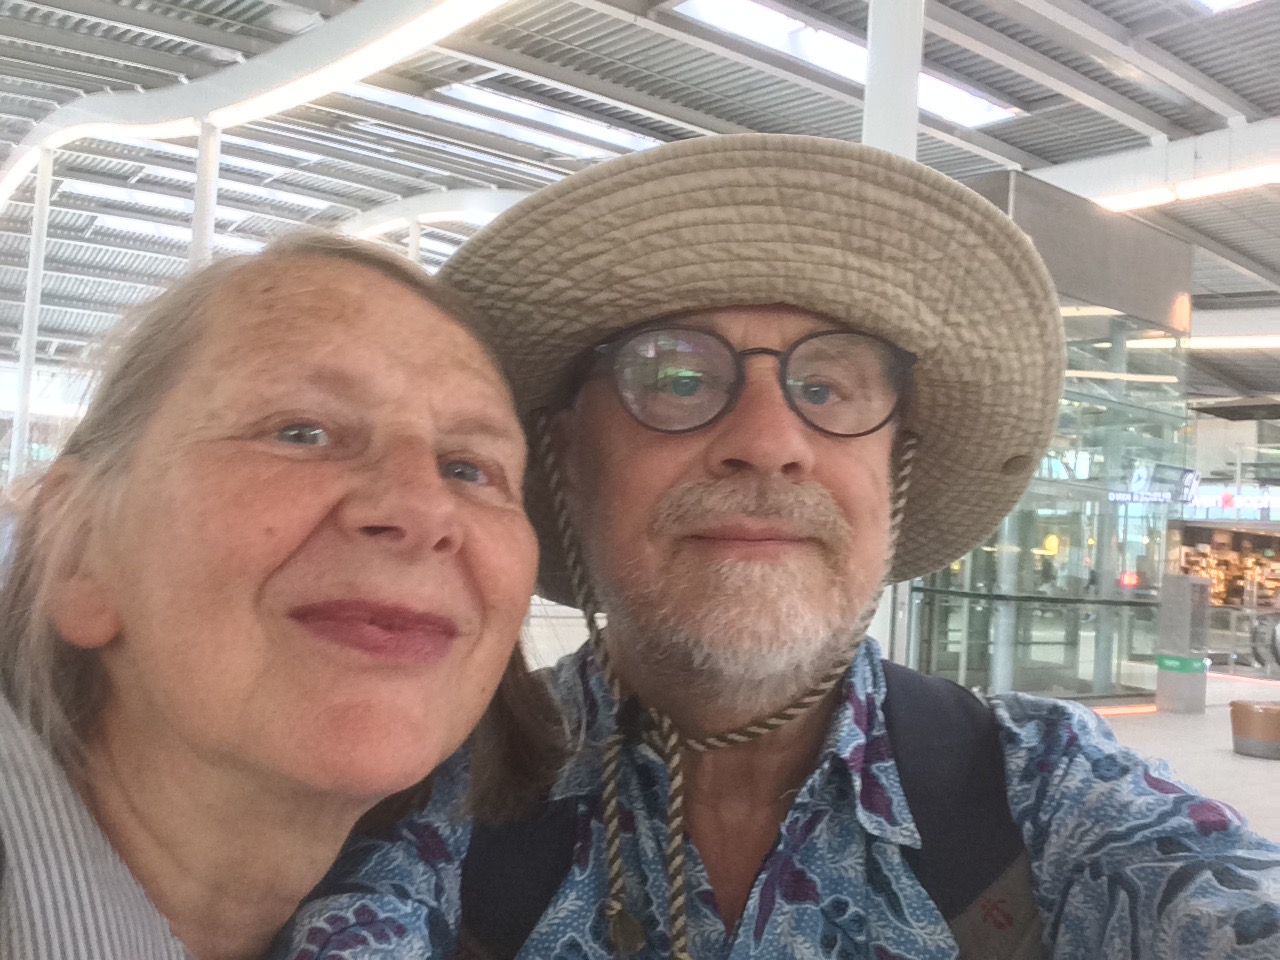
\includegraphics[width=0.9\columnwidth]{foto}
  \caption{On our way to Brazil}
\end{figure}

I did not expect to do any \TeX{} work, maybe some light programming,
for which I had a Python system
(Pythonista)\footnote{\url{http://omz-software.com/pythonista/}} on my
iPad.

While we were traveling in Brazil, on our way to Bolivia, I got an email
from a user of the \texttt{multirow} package about a possible bug. It
came with a solution which was a very simple substitution, and back home
on the laptop, it would have been a few minutes to make the change,
check it in into the version control system, do some test, generate a
new version of the documentation, and upload the new version to CTAN.

Because this person had already made a local change, and the problem was
not urgent anyway, my first reaction was: I will correct it when I am
back home, which, by the way, would be some 2 months later. However when
we arrived in Bolivia, where we were staying a couple of weeks, the
temptation to solve the problem right there became too large.

But what would have taken at most 10 minutes at home, became a major
effort without having a computer with a \TeX{} system. In the end it
took me more than two days of struggling, but with victory in the end.

If I would have distributed the package just as a collection of
\texttt{.sty} files (there are three included), with a separate
documentation, the task would have been simple. I could have downloaded
the package from CTAN, changed the \texttt{.sty} files with a text
editor in my iPad, and uploaded them back to CTAN. It might have caused
some frowning from the CTAN maintainers if the version number in the
documentation would have been different from the one in the
\texttt{.sty} files, but that would have been temporary anyway.

However, the package was distributed as a \texttt{.dtx} file, with a
corresponding \texttt{.ins} file, and a separate PDF file containing the
documentation which is generated from the \texttt{.dtx} file. The
\texttt{.sty} files are also generated from the \texttt{.dtx} file with
the aid of the \texttt{.ins} file. This is the standard setup for most
CTAN packages. But this requires the \texttt{.dtx} and \texttt{.ins}
files to be processed by \LaTeX{} (or \TeX{} in case of the
\texttt{.ins} file). And I did not have a \LaTeX{} distribution on my
iPad.

\begin{figure}
  \centering
  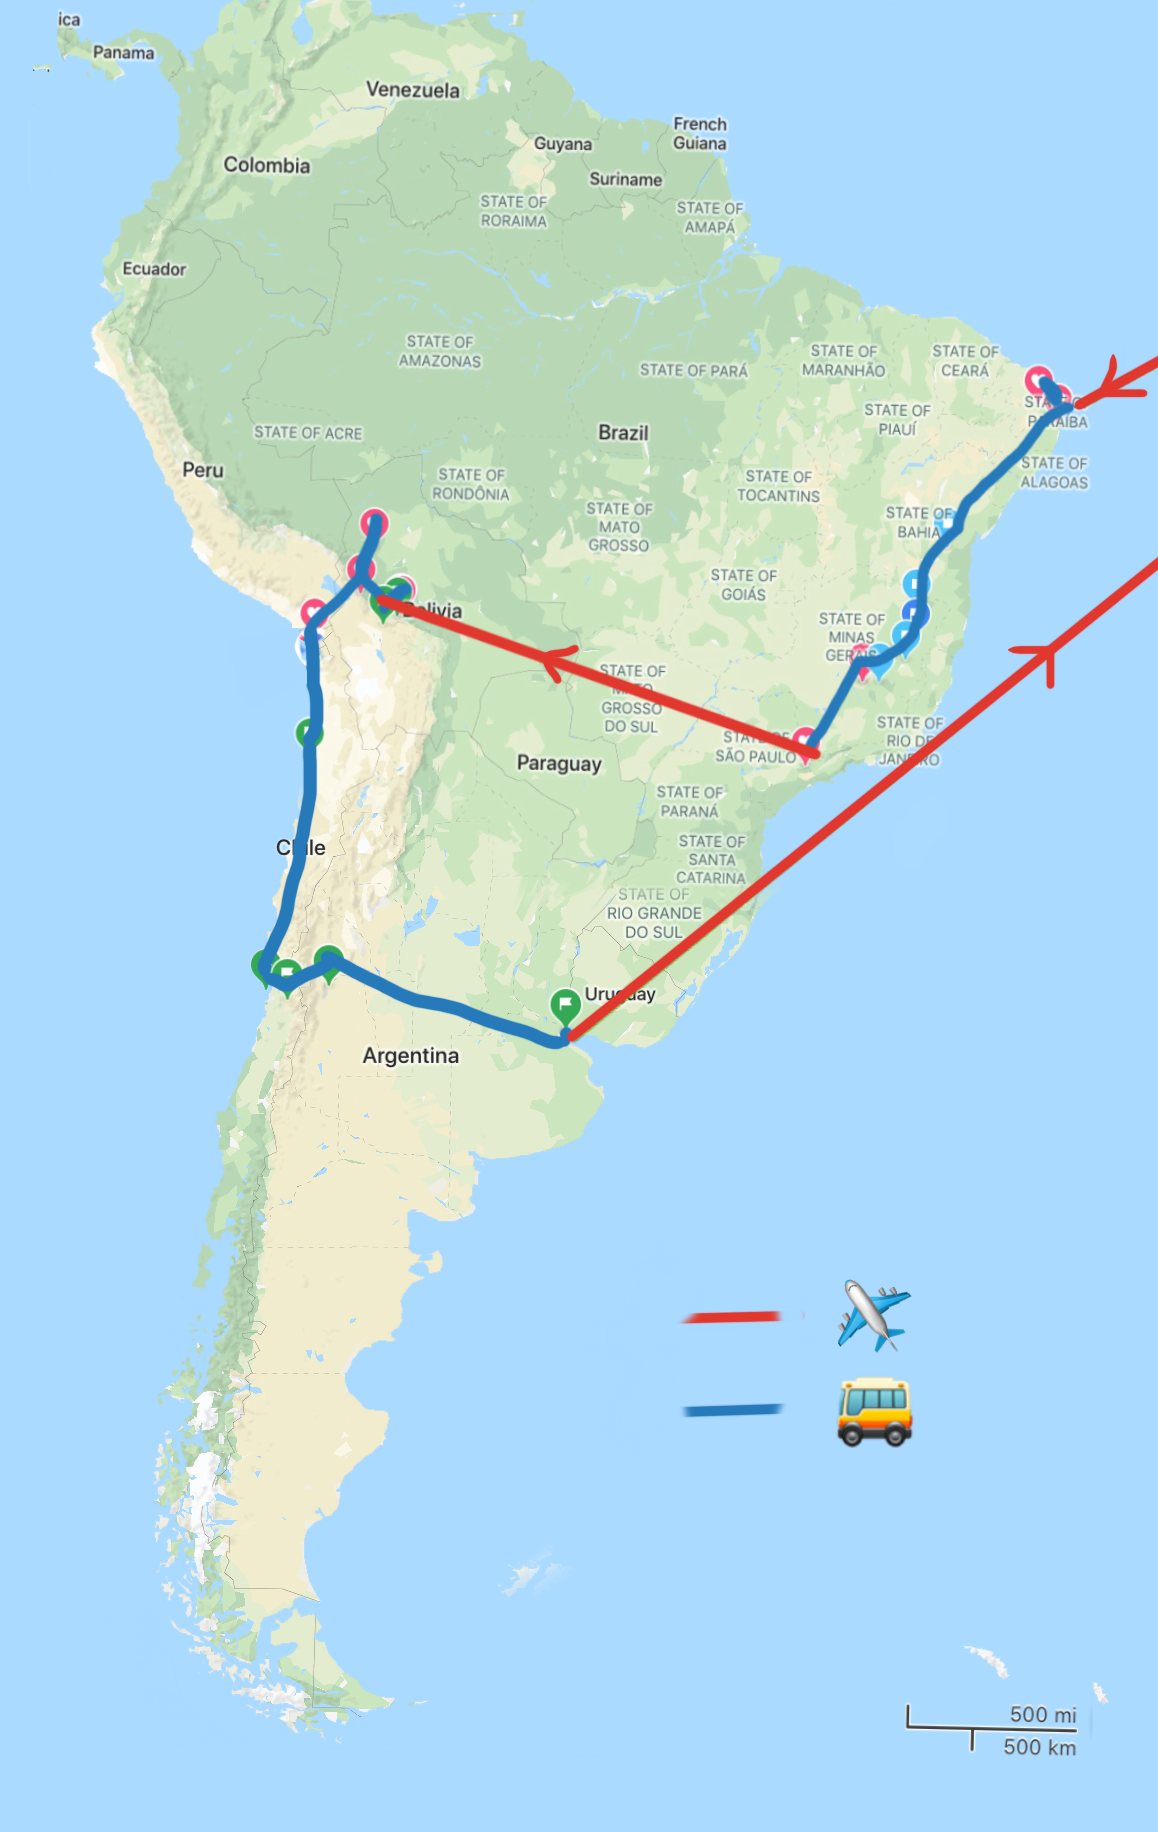
\includegraphics[width=0.9\columnwidth]{trip}
  \caption{Our trip}
\end{figure}

\section{What were the options?}

There were in practice two options to solve the problem:
\begin{itemize}
\item Install a \LaTeX{} system on my iPad.
\item Use an online (cloud-based) \LaTeX{} system.
\end{itemize}

\subsection{\LaTeX{} apps on the iPad}

I found two \LaTeX{} apps on the iOS App Store: Texpad and TeX Writer.
Both are offline apps, i.e.\ you don't need an internet connection to
compile your \LaTeX{} documents. But, on the other hand, in order to
limit the size of the application, they don't have every package from
CTAN installed. You can install additional packages, but as iOS is quite
a closed operating system, you are dependent on the developers to supply
these packages. Of course you have always the option to add the required
files to your project directory, but there might be some cases (for
example if you need additional fonts) that this is not sufficient.

Also it isn't clear from the documentation of these packages if they can
process something like \texttt{.dtx} and \texttt{.ins} files to extract
the \texttt{.sty} files and the documentation for the package, which was
essential in my case. I got the impression that they were mainly meant
for the `normal' user to write articles and reports.

They are also not particularly cheap. At this moment Texpad costs \euro
21.99 and TeX Writer \euro 16.99. If I remember correctly they were a
little bit cheaper at the time I was traveling. In itself that is not a
very steep price, but I did not expect to use it very often, and just
for this single case I thought it was too much. And they don't have a
tryout version to see if it really fits you, so if you buy one of these,
and you don't like it, you effectively lost your money. And then there
is this nagging choice: which of the two is best? All in all, I decided
not to go that way.

For the cloud-based systems, I had heard about Overleaf (formerly called
WriteLatex) and ShareLaTeX, so I decided to investigate these. It appeared
that at that time, these two systems were in a processed of being merged.
The result was Overleaf version 2 which had the ShareLaTeX interface, but
was still in beta phase. For the simple task that I had, a free account
would be sufficient, so I started to try that. However, the merging process
introduced some teething troubles. In fact it made editing the files from
the iPad browser almost impossible. It wasn't clear if this was a specific
problem on the iPad, or that the browser interface in general was not yet
mature enough. In effect it wasn't usable at all, because its behaviour was
very erratic.

I had also tried to use the Overleaf version 1 interface, but I also could
not get that working. I have no idea whether these problems were iPad
specific, but anyway I could not use it. By the way, the Overleaf editor is
now functioning also on the iPad. However, some functionality is not
available without an external keyboard, because they are invoked with
control keys. For example the search function is invoked by Control-F on
Windows and Linux, and by Command-F on MacOS. On an iPad you can't give
these with the virtual keyboard. With an external keyboard it is possible.
The current Overleaf editor is reasonable. It has some \TeX-specific
functionality. For example, if you type \verb|\begin{enumerate}| the editor
  adds \verb|\item| and \verb|\end{enumerate}| and positions the cursor
after the \verb|\item| (see figure~\ref{fig:enumerate}).
\begin{figure}[hb]
  \centering
  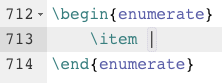
\includegraphics[width=0.9\columnwidth]{enumerate}
  \caption{Editor supplies useful parts}
  \label{fig:enumerate}
\end{figure}

\begin{figure}
  \centering
  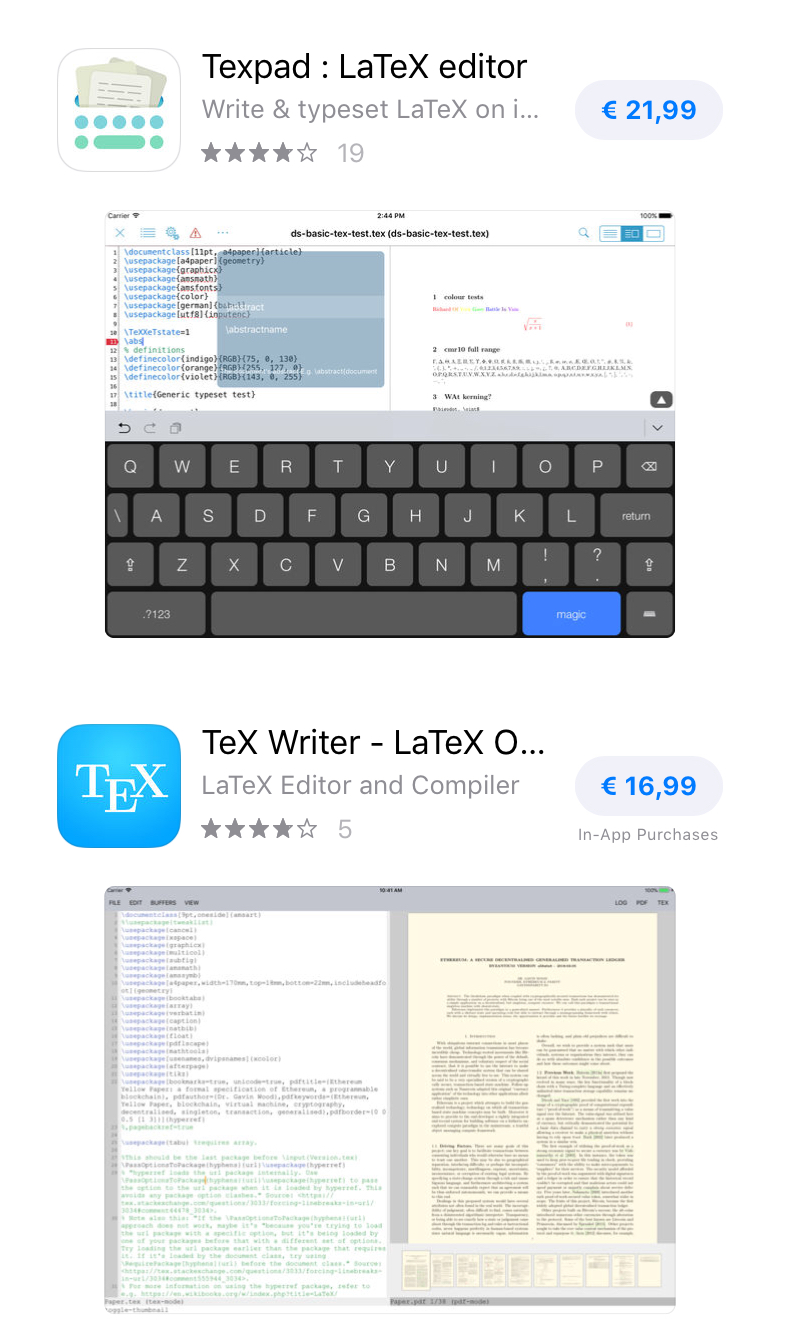
\includegraphics[width=0.9\columnwidth]{ios-apps}
  \caption{Texpad and TeX Writer in the iOS App Store}
\end{figure}

\subsection{Cloud-based \LaTeX{} systems}

\begin{figure*}
  \centering
  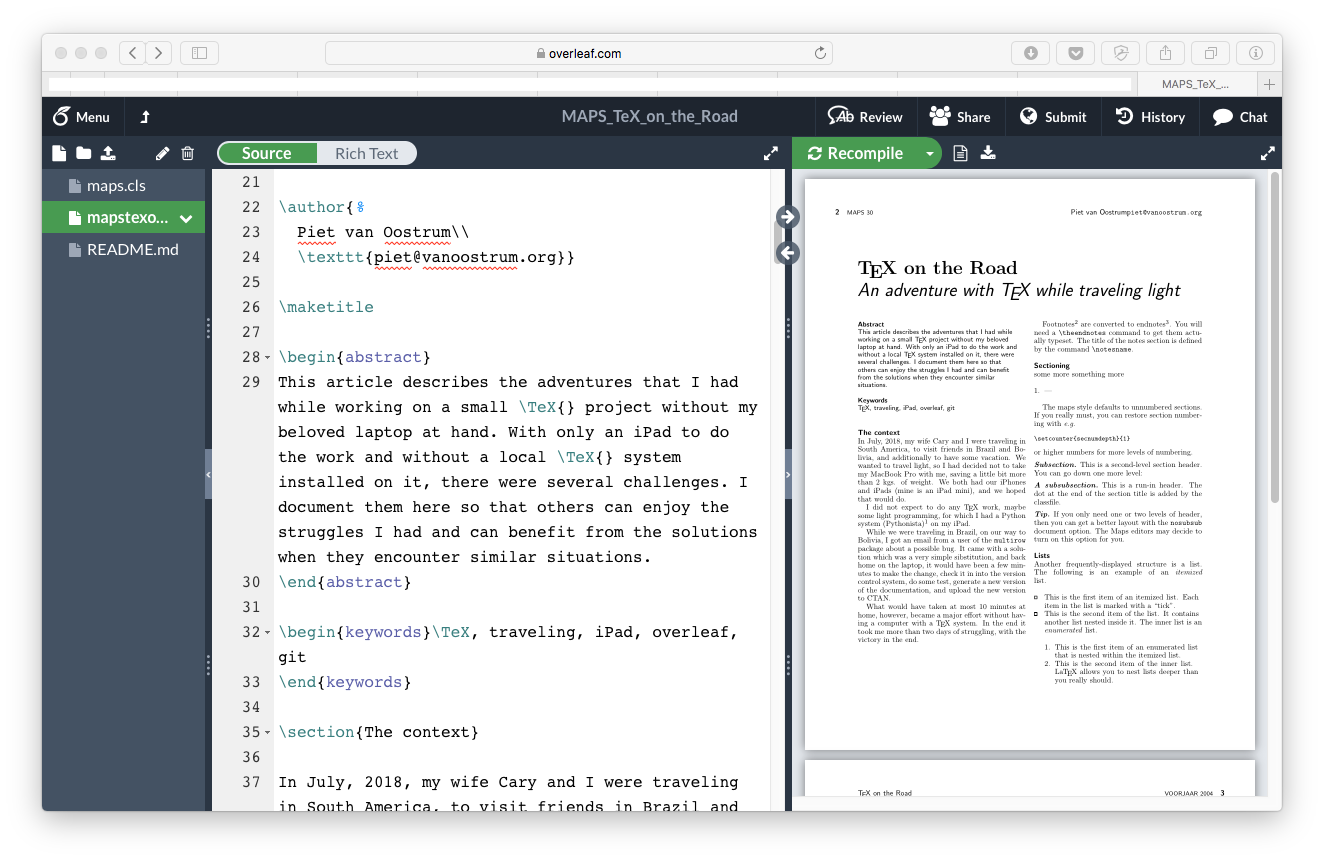
\includegraphics[width=0.75\textwidth]{overleaf}
  \caption{An early version of this article in Overleaf, with some of
    the maps.cls documentation still in place}\label{fig:overleaf}
\end{figure*}

\begin{figure*}
  \centering
  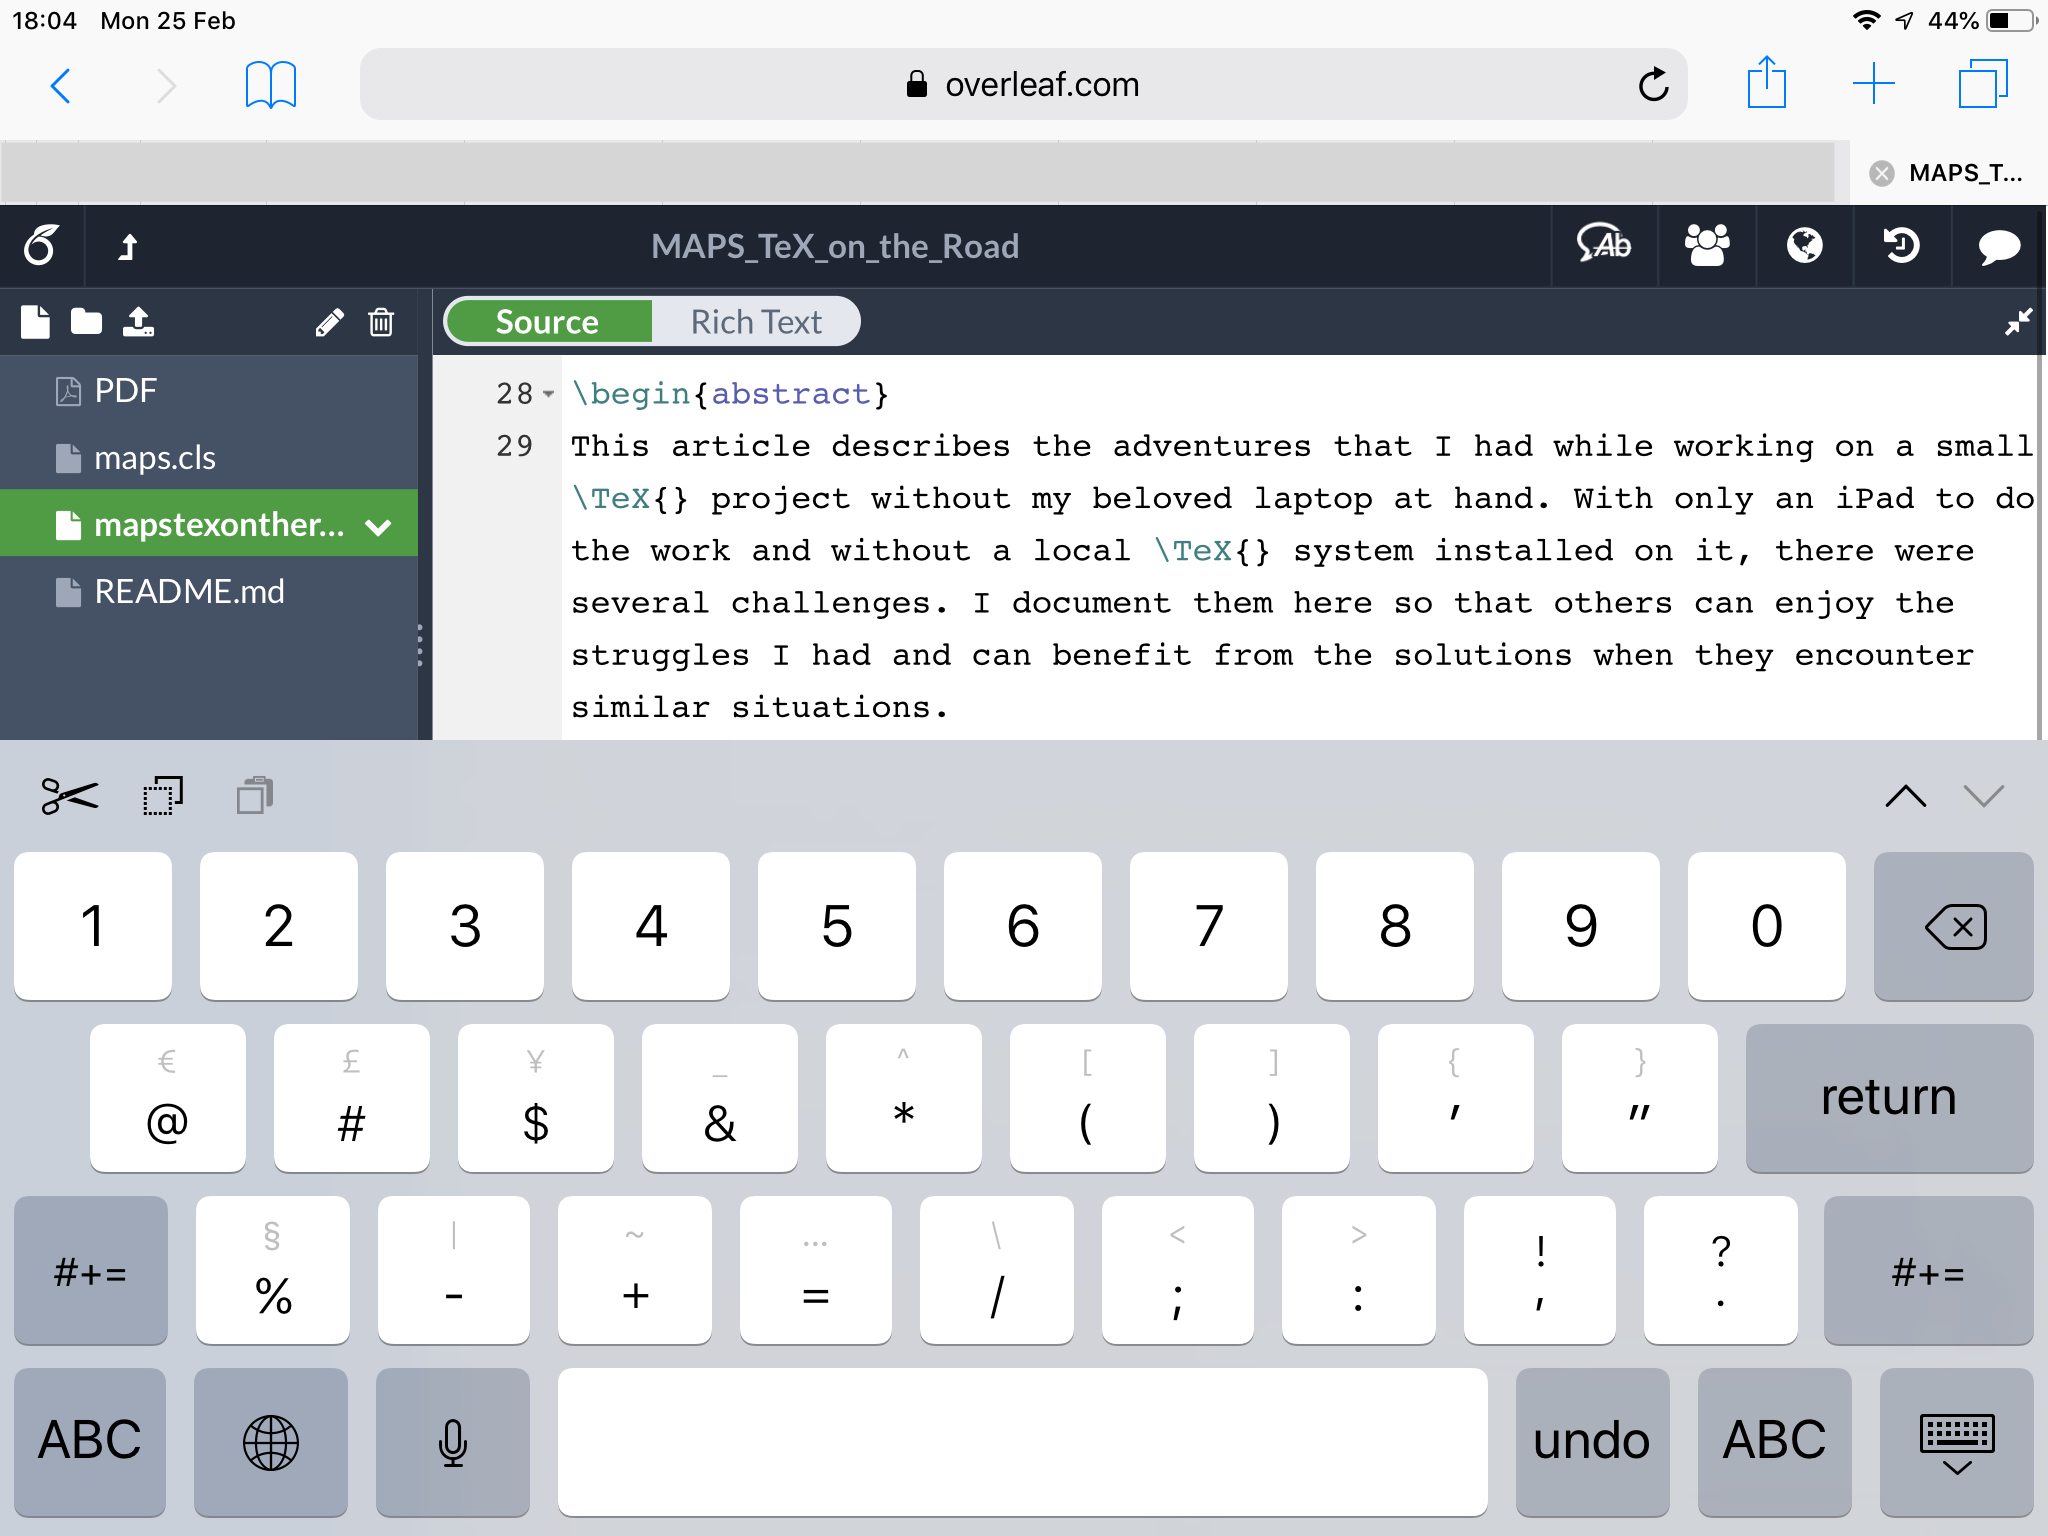
\includegraphics[width=0.75\textwidth]{overleaf-hor}
  \caption{Overleaf screen with virtual keyboard on an iPad}\label{fig:overleaf-hor}
\end{figure*}

\begin{figure*}
  \centering
  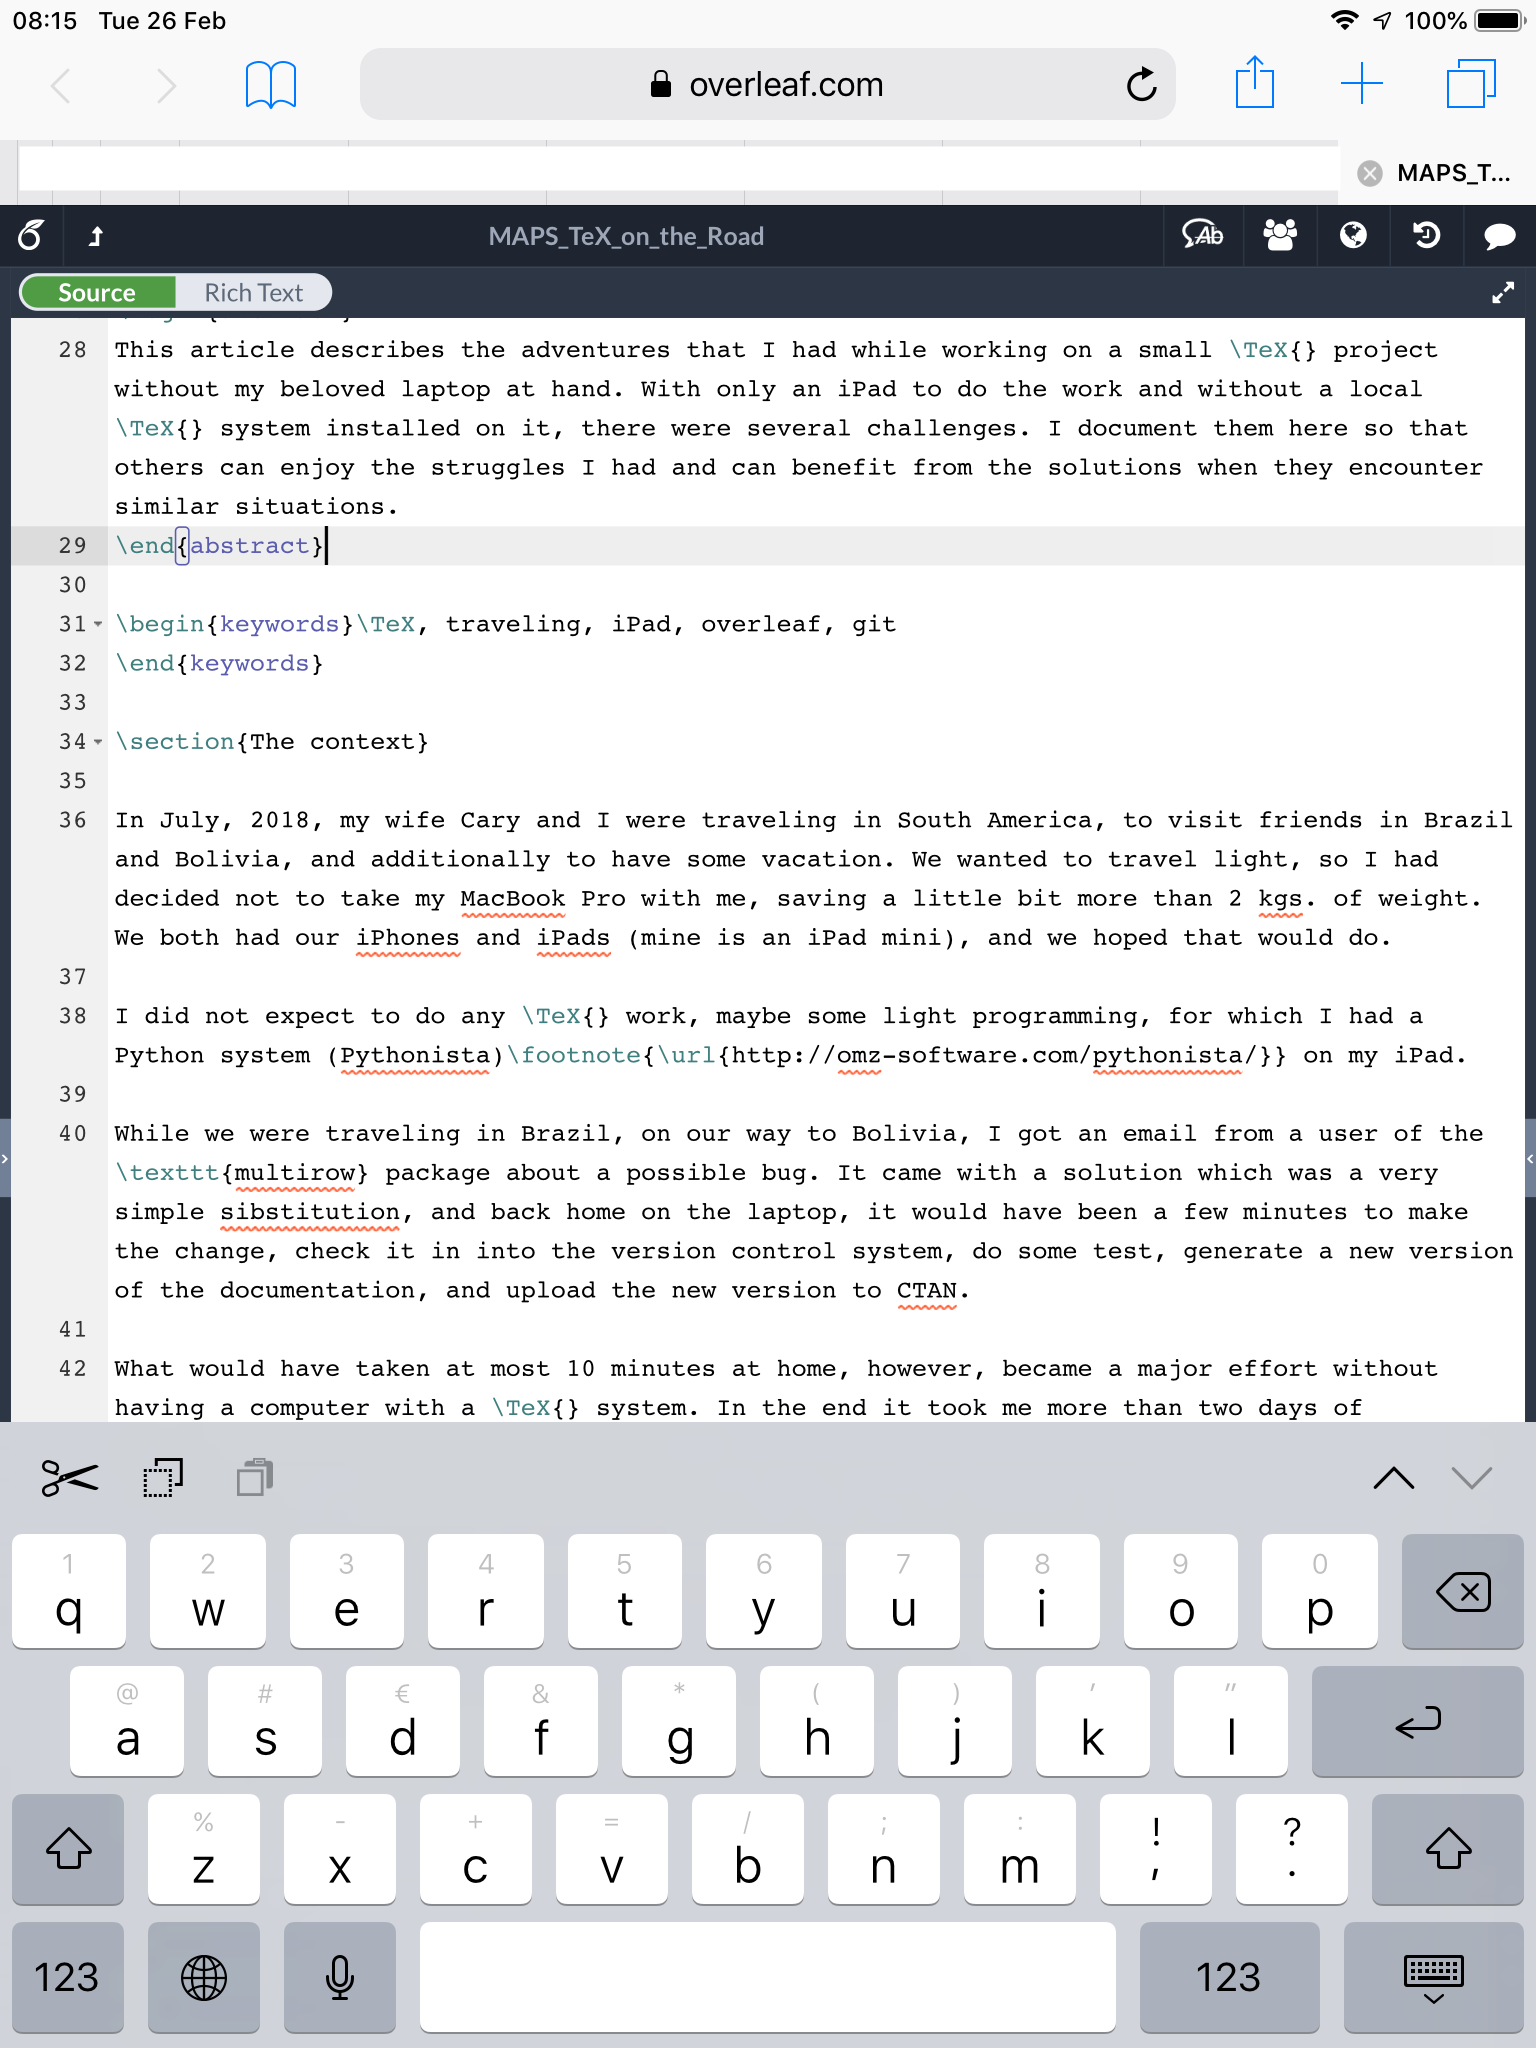
\includegraphics[height=0.75\textwidth]{overleaf-vert}
  \caption{Overleaf screen with virtual keyboard on an iPad in portrait
    mode}
  \label{fig:overleaf-vert}
\end{figure*}

\begin{figure*}
  \centering
  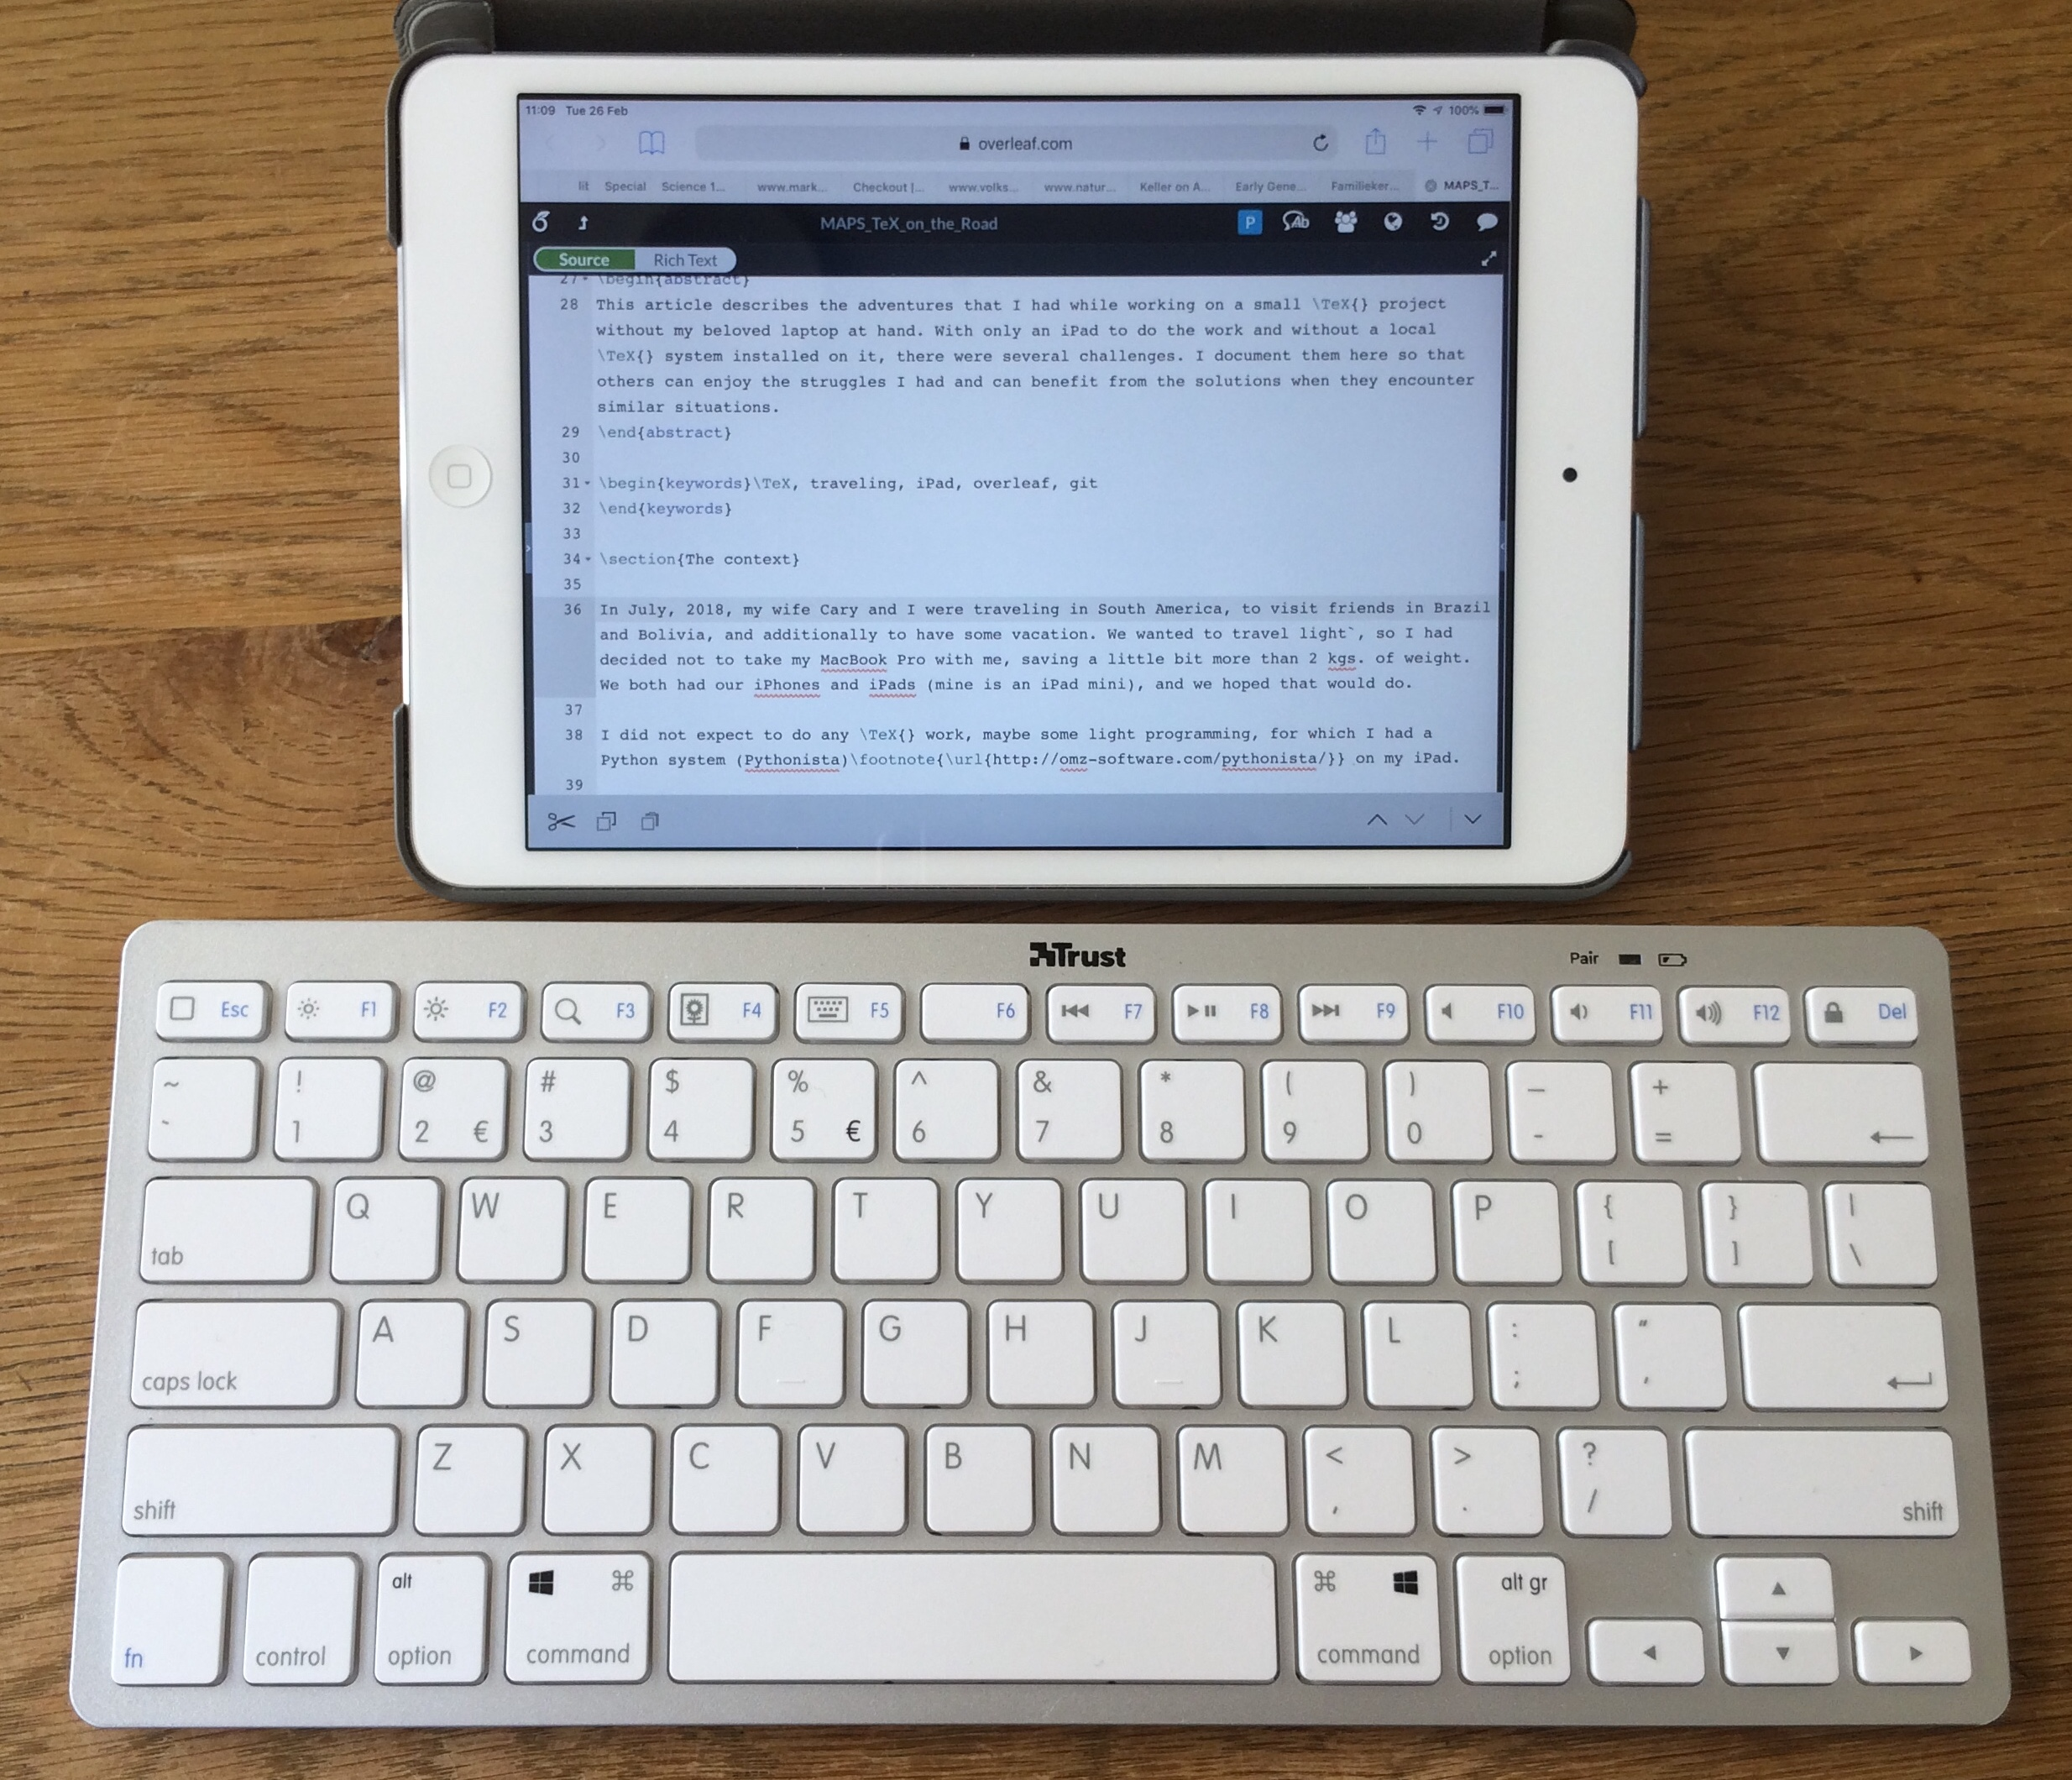
\includegraphics[width=0.75\textwidth]{iPad+keyboard}
  \caption{iPad mini with external keyboard}
  \label{fig:ipad+keyboard}
\end{figure*}

Despite the problems that the editor gave at that time, it seemed to me that
this was the best way to go forward. Figure~\ref{fig:overleaf} shows the
screen from the current version of Overleaf on my MacBook. The default
screen has an edit window with the \LaTeX{} source text and a preview window
with the resulting PDF. The preview is not live, you have to hit the
Recompile button to update it. There is also a file list on the left and it
has the possibility to hide or show each of these parts and to adjust the
sizes of each part. Especially on the smaller iPad screen it is advisable to
have only the source code part while editing. But even then, the virtual
iPad keyboard takes so much space the hardly any source code is visible. See
figure~\ref{fig:overleaf-hor}. Also in this case, the file list at the left
would make the edit window even smaller, but the file list can be hidden, as
shown in the image.

It helps to put the iPad in portrait mode, as shown in
figure~\ref{fig:overleaf-vert}. But then the keyboard is rather small. For a
setup like this to be workable, it would be better to use an external
keyboard. There are several keyboards on the market that can be used. They
are generally connected through Bluetooth. They are light-weight and don't
take much space, so ideal for traveling light. See
figure~\ref{fig:ipad+keyboard}. I did not have one at that moment, however.

\section{Setting up the project}

Setting up the project is easy. You can create a new project in the Overleaf
in the Web interface. You can upload each file individually, or a zipfile
with everything included. Overleaf will unpack the zipfile in your project.

Immediately, it became apparent that there was a problem with my project.
Overleaf wants you to designate one of your files as the main \TeX{} file,
which for me would have been \texttt{multirow.dtx}, but it doesn't accept
this. It wants to have a \texttt{.tex} file. It does not recognize the
\texttt{.dtx} file as a valid \LaTeX{} file. Neither does it want to edit
the \texttt{.dtx} file, but as the editor was unusable, this was of a minor
concern. I would have to edit the files locally on my iPad anyway.

So I had to give it a \texttt{.tex} file to make it (and myself) happy. I
tried two ways
\begin{itemize}
\item Copy \texttt{multirow.dtx} to \texttt{multirow.tex}
\item Make a file \texttt{multirow.tex} that just contains \verb|\include{multirow.dtx}|
\end{itemize}
I had expected that each of these would compile the \texttt{.dtx} file when
the Compile button would be pressed. However, it didn't. It took some time
to find out why. My \texttt{multirow.dtx} contains a line
\begin{verbatim}
\DocInput{\jobname.dtx}
\end{verbatim}
which is quite usual in \texttt{.dtx} files. After some searching I found
out that \verb|\jobname| wasn't \texttt{multirow} as was to be expected, but
\texttt{output}. It appears that Overleaf runs the job in a kind of
\emph{sandbox} where the jobname of the main file is \texttt{output}. You can see that in figure~\ref{fig:latexmkrc-debug}.

After some googling I found that Overleaf uses \texttt{Latexmk}\footnote{\url{}https://mg.readthedocs.io/latexmk.html} to process
the job. It provides a standard, but invisible, \texttt{latexmkrc} file that
controls the compilation process. However, you can also supply your
\texttt{latexmkrc} file. This file is described in
section~\ref{sec:latexmk}.

So the challenge was now to upload a correct \texttt{latexmkrc} file, and to
update the \texttt{multirow.dtx} file. This could be done by uploading these
files after each modification, but this might be an error-prone process, and
you don't have a record of what has been done. Enter \emph{version management}.

\section{Distributed version management}

In any project where you have to make changes more or less regularly, it is
important to keep track of what you have done. Also, in general it is useful
to have access to previous versions of your project, for example if you want
to go back to a previous situation. Some people do this by making copies of
their files at regular moments. Sometimes they put the date and the time in
the file names, to keep a kind of history. But this becomes soon unwieldy.
This is the problem that version management system (also called version
control systems) offer a solution for. Each serious developer, whether it is
of software or of texts, should consider using a version management system.

For those readers that are unfamiliar with version management, here follows
a brief description. You have a \emph{working copy} or \emph{working
  directory}, which is the collection of files that you work upon in your
project. This is just like when you do not use version management.
Additionally you have a \emph{repository}, which is a kind of database
containing the history of your project. It will contain the state of your
\emph{working copy} at certain moments in the past, together with
information about who made the changes, and a description of what has
changed.

If, at a certain moment, you have a state of your project that you want to
keep, you \emph{commit}, which means a copy is made to the
\emph{repository}, together with a description that you enter. The
opposite operation (i.e. making a copy from your repository to your working
directory) is called \emph{checkout}. You usually have a separate repository
for each project. The repository can be on your local computer, or on a
server. In the latter case it is possible that different people working on
the same project use the same repository. They would then each have their
own \emph{working copy}. As they are working independently, these could be
different. A version management system usually has provisions to resolve
conflicting working copies.

Although these systems can store any type of file, they work best with plain
text files. As our \TeX{} sources are plain text, they are ideal candidates
for using a version management system.

There are several version management systems available. One older,
well-known system is \emph{subversion}
(SVN\footnote{\url{http://subversion.apache.org}}). It usually has the
repositories at a central server, but you can also have the repository on
your local computer, if you are working alone. As SVN has only one
repository per project it is called a centralized version management system.

Centralized version management systems have some big disadvantages for
cooperation in teams:
\begin{itemize}
\item If you work together the repository must be on a central server, which
  means you cannot use it when you are offline.
\item If you want to keep your changes registered often in the repository,
  then this can be confusing for the other team members. On the other hand,
  if you want to keep the repository relatively clean, that is, only commit
  major updates, then you lose the possibility to keep your own history
  detailed.
\end{itemize}
One solution would be to have both a central repository for the team, and
your local repository for your own work, but then synchronizing these
repositories could become tedious. However, this is where \emph{distributed
  version management systems} have their strength.

In a \emph{distributed version management system} you can have both a local
repository on your computer and a central repository on a server. Or even
more than one of each. And these can be easily synchronized. The usual way
to work in a team is to have a central repository for the team, and a local
repository on each team member's computer. Each team member keeps a history
in the local repository. This can be done often, and also offline. When the
changes are good enough to be put in the central repository, the team member
\emph{pushes} the local changes to the central repository, often after
making one set of changes that do not reflect all the details of the work
done locally. Other team member can the \emph{fetch} these changes from the
central repository when they want to be up-to-date. It is then probable that
this is not consistent with some changes that they made themselves. The two
sets of changed must then be \emph{merged}. This is the simple explanation.
Much more complicated workflows are also possible.

Both centralized and distributed version management systems support the
concept of \texttt{branches}. A \texttt{branch} is a separate line of
development in your project. For example you have a project that you release
from time to time. The development of this release version would for example
take place on the main branch in your repository. Now after a release you
want to start working on some very new experimental features for a fxuture
release. If you would just continue your development, then when a bug in
your project is detected, your project is in an unstable state. So you
cannot just apply a bug-fix to the current state of your project, but you
would have to go back to the state just after the release. As the repository
has kept the history of your project, this is easy, but you want also to
keep the current state, so that you can go back there after making the
bug-fix. Here branches come to the rescue. After your release you create a
new branch for your experimental work, and continue working there. When you
want to make the bug-fix, you switch back to the main branch. The repository
will remember your experimental branch, and after releasing the bug-fix you
can switch back to the experimental branch. If you wish you can then also
\emph{merge} the fix in your experimental branch. Later when your experiment
is successful and you want to release it, you can merge it back to the main
branch. You can have as many branches as you want. For example if your
bug-fix is expected to be complicated, you can first try it out on a
separate branch.

A very popular site for central repositories is
Github.\footnote{\url{https://www.github.com}} This site is based on the
distributed version management system \texttt{Git}. Git is probably the most
popular version management system in use today. For my own projects I use
Git exclusively nowadays, often only locally, but sometimes in combination
with Github.

\subsection{Use with Overleaf}

To come back to the project I am currently describing, it appeared that
Overleaf also had Git possibilities. Although these were in beta phase at
that moment, it could be used for my project. Nowadays you need a paid
account on Overleaf to use the Git facilities, but because I had started
using them during the beta testing, I have access to them in my free
account.

Git can be used in two ways on Overleaf.
\begin{itemize}
\item Your Overleaf project can function as a Git repository
\item You Overleaf project can be synchronized with a Github repository
\end{itemize}

I decided to take the Github route, mainly because I have experience with
Github and I could not get the direct Git repository on Overleaf working
from the iPad. At this moment it is working, but its functionality is very
minimalist compared to Github.

In order to use Git on the iPad you need a Git app. I found
Git2Go,\footnote{\url{https://git2go.com}} which is said to be the first app
to use Git on iOS. It worked well for my needs, but later I tried two others
that I found: Working Copy\footnote{\url{https://workingcopyapp.com}} and
TIG.\footnote{\url{https://itunes.apple.com/us/app/tig-git-client/id1161732225}}
In the appendix I give a comparison of these apps.

\begin{figure}
  \centering
  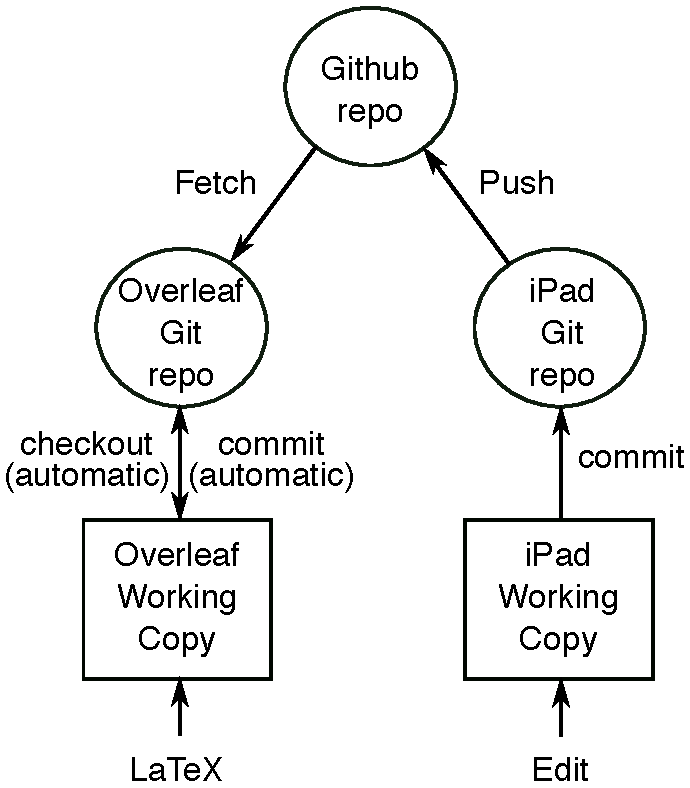
\includegraphics[width=0.9\columnwidth]{Git}
  \caption{Git workflow}
  \label{fig:git}
\end{figure}

My workflow can be found in figure~\ref{fig:git}. My editing took place in
the lower right corner, on the working copy (managed by Git2Go). I could
have used the editor that Git2Go provides, but it is not very sophisticated.
It does not have syntax highlighting for \LaTeX{} files, and it gives no
editing support beyond the standard iPad keyboard. I also had e much better
text editing program called
Textastic\footnote{\url{https://www.textasticapp.com}}. It has syntax
highlighting for \LaTeX{}, good search facilities and an extended keyboard
that makes it easier to enter non-alphanumeric symbols. Also it has a
special provision for easy cursor movement. Git2Go, and the other Git apps mentioned above, function as a kind of file system, which means that Textastic can directly edit their files without copying between the two apps. So the only extra operation to edit in Textastic rtather than in Git2Go itself, is switching between the apps. This extra effort I deemed worthwhile for the added comfort of using a good text editor.

After editing the file(s), I switch to Git2Go, commit the change, and immediately push it to the Github repository. Then I switch to Overleaf in the browser, fetch the changes from Github to Overleaf in the Overleaf synchronization menu, and process the files, hopefully producing a new PDF file. Many times it did not yet work correctly, so I had to go back to Textastic and start a new cycle. The problem wasn't so much in the \LaTeX{} code, as the changes there were very simple. The main problem was getting the \texttt{latexmkrc} file correct. The difficulty was that Overleaf did not have good documentation about the context in which the Latexmk program was running. Also, running it on their server did not give as much feedback as running on your own computer. Several times I had to write extra information to a text file, and then download that to the iPad to see what happened. For example, I had to make directory listings, and write them to a text file, just to see what files where generated and what their names were. And the process was a bit tedious because I had to synchronize the files as described above before each try. But after some 50 tries, everything worked perfectly. I will spare you all the attemts that I made, but in the next section I will give you the resulting \texttt{latexmkrc} file, and explain what it does.

\section{Latexmk}
\label{sec:latexmk}

\begin{figure*}
\textbf{Latexmkrc file:}
\begin{Verbatim}[numbers=left,xleftmargin=7mm]
$ENV{'TZ'} = 'America/La Paz';

add_cus_dep('glo', 'gls', 0, 'makeglo2gls');
sub makeglo2gls {
    system("makeindex -s gglo.ist -o \"$_[0].gls\" \"$_[0].glo\"");
}

$makeindex = 'makeindex -s gind.ist -o %D %S';

push @generated_exts, 'glo', 'gls', 'glg', 'sty', 'txt';

$pdflatex = 'internal mylatex';
sub mylatex { 
    my @args = @_;
    (my $base = $$Psource) =~ s/\.[^.]+$//;
    system("tex $base.ins");
    # backslashes are interpreted by (1) perl string (2) shell (3) sed regexp
    # therefore we need 8 backslashes to match a single one
    system("sed -e s/\\\\\\\\jobname/$base/g $base.dtx > $base.tex");
    return system("pdflatex @args");
}
\end{Verbatim}
  \caption{The final latexmkrc file. The line numbers are not part of the file.}\label{fig:latexmkrc}
\end{figure*}

Latexmk is a program (a Perl script) to process a \LaTeX{} file with all the necessary \texttt{bibtex}, \texttt{makeindex} and similar calls. It will run \LaTeX{} and these other programs as many times as is necessary to get a completely processed and stable output.
For the run-of-the-mill \LaTeX{} file, Latexmk has enough knowledge to know what to do. However, when there are additional requirements, like a non-standard index, glossaries etc.\ you must give Latexmk a recipe of how to process the various stages. The recipe is given in the \texttt{latexmkrc} file, which in fact is also a Perl script. Latexmk has an enormous amount of possibilities, and its manual\footnote{\url{http://mirrors.ctan.org/support/latexmk/latexmk.pdf}} contains 48 pages. So it took some time to get everything right.

Overleaf provides a standard \texttt{latexmkrc} file for its jobs, but as we have seen above, this is not adequate for processing the \texttt{.ins} and \texttt{.dtx} files. To make Overleaf happy, we must provide a main \texttt{.tex} file, but with our \texttt{latexmkrc} file we don't use it, so its content is unimportant.

In figure~\ref{fig:latexmkrc} the resulting \texttt{latexmkrc} for this process is given, annotated with line numbers. In the remainder of this section I explain what it does.
\begin{descript}
  \item[line 1.] This sets the timezone to your local time. This is so
  that messages with date and time will get your local time, and not the
  time of Overleaf's servers, which would be useless in most cases. As I
  was in Bolivia at the time, the timezone was 'America/La Paz'. Now at
  home it would be 'Europe/Amsterdam'.

  \item[line 3-6.] In a \texttt{.dtx} file the file extension
  \texttt{.glo}, which is normally used for glossaries, is used for the
  list of changes. And the sorted version, to be created by
  \texttt{makeindex}, will be \texttt{.gls}. These lines give a recipe
  how to create the \texttt{.gls} file from the \texttt{.glo} file using
  \texttt{makeindex}.

  \item[line 8.] For processing the normal index in a \texttt{.dtx}
  file \texttt{makeindex }needs the additional argument
  \texttt{-s~gind.ist}.

  \item[line 10.] This defines which extra file extensions we need in
  the process. Besides the already mentioned \texttt{.glo} and
  \texttt{.gls}, there is also \texttt{.glg} which is the log output of
  the \texttt{makeindex} command from line 5. And the \texttt{.txt}
  extension is used for debugging.

  \item[line 12.] Here comes the trick to let Overleaf do our work.
  Normally it will run \texttt{pdflatex} on the main \TeX{} file, which
  in our case is \texttt{multirow.tex}. But you can define the
  \texttt{\$pdflatex} variable to let it use another command. In our
  case we let it run the internal function \texttt{mylatex} that
  follows. In this function we do all the preparatory work before we run
  the actual \texttt{pdflatex}.

  \item[line 14.] Pick up the arguments from the call to
  \texttt{mylatex} in the variable \texttt{@args}. This is standard Perl
  prose.

  \item[line 15.] Latexmk puts the name of the main \TeX{} file in
  \texttt{\$\$Psource} (see page~45 in the Latexmk manual). This line is
  actually a shorthand for two statements:
\begin{verbatim}
my $base = $$Psource;
$base =~ s/\.[^.]+$//;
\end{verbatim}
  The first line copies \texttt{\$\$Psource} to a local variable
  \texttt{\$base}. The second line strips of the part after (and
  including) the last dot. So \texttt{multirow.tex} will be transformed
  to just \texttt{multirow}. The reason I use \texttt{\$\$Psource}
  rather than just using \texttt{multirow} is that now the
  \texttt{latexmkrc} file is also usable for other \texttt{.dtx} files.

  \item[line 16.] First we run \texttt{tex} on our \texttt{.ins}
  file, which would be \texttt{multirow.ins} in our case. This generates
  the required \texttt{.sty} files. This is to ensure that we use the
  new versions of our \texttt{.sty} files, rather than an outdated
  version in Overleaf's \TeX{} system.

\item[line 19.] From our \texttt{.dtx} file we generate a copy to our
  \texttt{.tex} file where the text \verb|\jobname| is replaced by the
  actual base name of our file (in our case \texttt{multirow}). This is
  necessary, as Overleaf supplies a \verb|\jobname| of \texttt{output}.
  So in this case we generate \texttt{multirow.tex} from
  \texttt{multirow.dtx}. But this file will input \texttt{multirow.dtx} during its processing.

  We do the replacement by calling the Unix program \texttt{sed}. The
  \verb|\jobname| is inside a regular expression in \texttt{sed},
  therefore the backslash must be doubled. But then, this command is
  processed by the Unix shell, which also interprets backslashes.
  Therefore we must double all the backslashes again. And then this
  command is inside a Perl string where backslashes are also
  interpreted. So we must double them again, and we end up with 8
  backslashes to represent a single one.

\item[line 20.] Finally we run the real \texttt{pdflatex} command with
  the original arguments. Note that we process the new
  \texttt{multirow.tex} file, because that is what Overleaf expects to
  do. Also, because this is run in a \texttt{sandbox} (i.e. on a copy of
  the original files in a separate directory), this does not affect our
  original file.
\end{descript}

Finally, we also give an example of the \texttt{latexmkrc} file with debugging statements included in figure~\ref{fig:latexmkrc-debug} and the corresponding output in figure~\ref{fig:debug-output}.
You see the values of \texttt{\$\$Psource} and \texttt{\$base}, the arguments to the \texttt{pdflatex} call, and the directory listing at the end of the process. Please note that
in the directory listing there is a file \texttt{multirow.log}; this is the result of the call \texttt{tex~multirow.ins}. Note also the generated \texttt{.sty} files. 
The files resulting from the \texttt{pdflatex} call on \texttt{multirow.tex/dtx} are all called \texttt{output.*}.
So \texttt{makeindex} must also act on these files. In figure~\ref{fig:latexmkrc}, line~5, this is accomplished because the file name is given as argument to the function makeglo2gls. In line~8 it is accomplished because the patterns \texttt{\%S} and \texttt{\%D} are replaced by the \emph{source} and \texttt{destination} of the command, respectively. I.e. \texttt{output.idx} and \texttt{output.ind}.

\begin{figure*}
\textbf{Latexmkrc with debugging:}
\begin{verbatim}
$ENV{'TZ'} = 'America/La Paz';

add_cus_dep('glo', 'gls', 0, 'makeglo2gls');
sub makeglo2gls {
    system("makeindex -s gglo.ist -o \"$_[0].gls\" \"$_[0].glo\"");
}

$makeindex = 'makeindex -s gind.ist -o %D %S';

push @generated_exts, 'glo', 'gls', 'glg', 'sty', 'txt';

$pdflatex = 'internal mylatex';
sub mylatex { 
    my @args = @_;
    Run_subst("echo \"%%B=%B %%R=%R %%S=%S %%T=%T\" > debugout.txt"); ## DEBUG ##
    system("echo '\@args' = \"@args\"              >> debugout.txt"); ## DEBUG ##
    system("echo '\$\$Psource' = \"$$Psource\"     >> debugout.txt"); ## DEBUG ##
    (my $base = $$Psource) =~ s/\.[^.]+$//;
    system("echo '\$base' = \"$base\"              >> debugout.txt"); ## DEBUG ##
    system("tex $base.ins");
    # backslashes are interpreted by (1) perl string (2) shell (3) sed regexp
    # therefore we need 8 backslashes to match a single one
    system("sed -e s/\\\\\\\\jobname/$base/g $base.dtx > $base.tex");
    $status = system("pdflatex @args");
    system("ls -l                                  >> debugout.txt"); ## DEBUG ##
    return $status;
}
\end{verbatim}
  \caption{\texttt{latexmkrc} file with debug statements}
  \label{fig:latexmkrc-debug}
\end{figure*}

\begin{figure*}
\textbf{Debug Output:}
\begin{verbatim}
%B=output %R=output %S=multirow.tex %T=multirow.tex
@args = -synctex=1 -interaction=batchmode -recorder -output-directory=/compile --jobname=output multirow.tex
$$Psource = multirow.tex
$base = multirow
total 1176
-rw-r--r-- 1 tex tex   3871 Mar  4 14:12 README
-rw-r--r-- 1 tex tex     49 Mar  4 14:12 README.md
-rw-r--r-- 1 tex tex   1417 Mar  4 14:12 bigdelim.sty
-rw-r--r-- 1 tex tex   1234 Mar  4 14:12 bigstrut.sty
-rw-r--r-- 1 tex tex    203 Mar  4 14:12 debugout.txt
-rw-r--r-- 1 tex tex   1054 Mar  4 14:12 latexmkrc
-rw-r--r-- 1 tex tex  80398 Mar  4 14:12 multirow.dtx
-rw-r--r-- 1 tex tex   2182 Mar  4 14:12 multirow.ins
-rw-r--r-- 1 tex tex   3719 Mar  4 14:12 multirow.log
-rw-r--r-- 1 tex tex   5022 Mar  4 14:12 multirow.sty
-rw-r--r-- 1 tex tex  80398 Mar  4 14:12 multirow.tex
-rw-r--r-- 1 tex tex   3487 Mar  4 14:12 output.aux
-rw-r--r-- 1 tex tex      0 Mar  4 14:12 output.chktex
-rw-r--r-- 1 tex tex  25207 Mar  4 13:10 output.fdb_latexmk
-rw-r--r-- 1 tex tex  20593 Mar  4 14:12 output.fls
-rw-r--r-- 1 tex tex   3281 Mar  4 14:12 output.glo
-rw-r--r-- 1 tex tex   3578 Mar  4 08:13 output.gls
-rw-r--r-- 1 tex tex   3270 Mar  4 14:12 output.idx
-rw-r--r-- 1 tex tex    891 Mar  4 08:13 output.ilg
-rw-r--r-- 1 tex tex   2655 Mar  4 08:13 output.ind
-rw-r--r-- 1 tex tex  34086 Mar  4 14:12 output.log
-rw-r--r-- 1 tex tex 610336 Mar  4 14:12 output.pdf
-rw-r--r-- 1 tex tex 262970 Mar  4 14:12 output.synctex.gz
-rw-r--r-- 1 tex tex   1467 Mar  4 14:12 output.toc
\end{verbatim}
  \caption{\texttt{latexmkrc} debug output}
  \label{fig:debug-output}
\end{figure*}

\section{Conclusion}



\appendix
\section{Appendix -- iOS Git apps compared}
\label{sec:appendix}

In this section I compare the three Git apps on iOS that I tried. I did all the production work in Git2Go, but after it was finished I also tried Working Copy and TIG.
  
\begin{descript}
\item[Git2Go] has a limitation that it only cannot work with Git repositories
  on all servers. It works with a limited number of services, namely
  Github, Bitbucket\footnote{\url{https://bitbucket.org}} and
  Gitlab\footnote{\url{https://gitlab.com}}. Other remote repositories
  can be used if they offer access by the SSH protocol. SSH is one of
  the two main protocols used to connect to Git servers. The other is
  HTTPS. Overleaf only offers HTTPS, which Git2Go does not support.

  To create a repository on your iPad you must \emph{clone} (i.e. copy) an existing repository on one of the supported servers. You cannot create a local-only repository on the iPad. Once you have the repository on your iPad, you can edit the files in the repository, commit the changes, create new branches. It can fetch from  and push to the remote repository, but these are not separate operations. It always does a fetch (which may be empty), followed by a push. It can also merge different branches. It is a limited set of operations compared to the full Git functionality, but it is sufficient for a normal workflow as described above. Also cooperating with other people would be possible, if it doesn't require the more esoteric Git functionality. Git2Go's editor has syntax highlighting for a limited number of programming languages.

Git2Go is free, as long as you only access \emph{public} repositories (i.e. repositories that everybody can see). To access private repositories you would have to buy an upgrade.

For the push operation you will have to login, and Git2Go will remember your username and password, until you explicitly logout.

And occasionally it crashes.

\textbf{Last minute Note:} I tried to re-install Git2Go on my iPhone, and got the message that it was no longer available on the App Store. Also a search in the App Store did not come up with Git2Go. I have no idea if this is a permanent situation, or that it might be in a process of updating.

\item[Working Copy] is the nicest of the three apps. It has a very elaborate set of functions. It can connect to all kinds of servers, including Overleaf. However, to use the \texttt{push} functionality you have to pay. The price is quite steep (\euro 17.99 at the time of writing), but you can get a free 10 day trial. I used this for writing this article to see how it worked.

Working Copy can clone from existing repositories, including through SSH and HTTPS, and also create local repositories. It can also create a local repository from a \texttt{.zip} file. Once you have a repository it can  connect your repository to more than one remote repository, which sometimes can be quite handy. For example in the current example, the repository on the iPad could have been connected both to the Overleaf repository and to the Github repository. Of course you will have to be careful not to mess up your workflow. 

If your iPad is connected to a Mac or PC with iTunes, you can drag and drop a repository on your computer through iTunes, and it will be copied to the iPad.

Working Copy's editor has syntax highlighting for  more than 50 different languages. It can show nice graphical representations of your branches and you commit history. Besides the \texttt{merge} functionality it also has the \texttt{rebase} functionality, which is an alternative for merge. For cooperating in large projects this functionality is sometimes necessary.

There is more than fits in this limited space, but Working Copy is far out the best of the three apps. It is expensive, but when you do a lot of work with Git on your iPad, it is worth the price. Working Copy operates in a small market, so the price is understandable. If you reaaly want to do serious work with Git on your iPad, it is recommendable to buy this app.

\item[TIG] is the third app I tried. It takes more or less a middle ground between Git2Go and Working Copy. Like Working Copy it can connect to all kinds of repositories, including Overleaf, and it has \emph{push} functionality. And it is free. It can clone existing repositories, and create local ones. It can also connect repositories to more than one remote repository.

Its editor has syntax highlighting support for 166 languages.

However, although the functionality is great for a free app, I found its user interface sometimes confusing. And to fetch/push to your remote repositories you have to enter your username and password every time. I did not find a way in which it could remember these. This is very annoying.
And it crashed quite often.
\end{descript}

Summary:
\begin{itemize}
\item If you only need access to repositories hosted by Github,
  Bitbucket or Gitlab, or repositories that can be accessed by the SSH
  protocol, and your requirements are modest, you can choose Git2Go (if
  still available).
\item If you need access to repositories that do not fall in the
  previous categories (such as Overleaf), and you can live with a not so
  optimal user interface, and your requirements are modest, you can
  choose TIG. It may be a good choice when you
  want to connect to a repository that Git2Go does not support, and when
  you find Working Copy too expensive.
\item If you want the top Git app on your iPad (or iPhone) and are
  willing to pay the price, I would recommend Working Copy. If you want
  to do serious work with Git, this is the choice and it would be worth
  the price.
\end{itemize}
There are nowadays some other Git apps available, but it seems that they are roughly comparable to one of the above. 

\theendnotes

\end{document}
